% Copyright (C)  2015  Alexander Jankowski, Philipp Hacker.
% Permission is granted to copy, distribute and/or modify this document
% under the terms of the GNU Free Documentation License, Version 1.3
% or any later version published by the Free Software Foundation;
% with no Invariant Sections, no Front-Cover Texts, and no Back-Cover Texts.
% The lincense itself can be found at <https://www.gnu.org/licenses/fdl-1.3>.

\documentclass[numbers=noenddot,a4paper,notitlepage,twoside,BCOR15mm]{scrartcl}
%\documentclass[numbers=noenddot,12pt,a4paper]{scrartcl}

\usepackage{ifoddpage}
\usepackage[infoshow]{tabularx}
\usepackage{fancyhdr}
\usepackage[greek,ngerman]{babel}
\usepackage[T1]{fontenc}
\usepackage[utf8]{inputenc}
\usepackage{libertine}
\usepackage{ziffer}
\usepackage{graphicx}
\usepackage{units}
\usepackage[infoshow]{tabularx}
\usepackage[all]{xy}
\usepackage{amsmath}
\usepackage{amssymb}
\usepackage{wrapfig}
\usepackage{upgreek}
\usepackage{esint}
\usepackage{float}
\usepackage[font=small,labelfont=bf]{caption}
\usepackage{subcaption}
\usepackage{lscape}
\usepackage[backref=page]{hyperref}
\usepackage{cleveref}
\usepackage{csquotes}

\renewcommand{\headrulewidth}{0.1pt}
\renewcommand{\footrulewidth}{0.1pt}
\newcommand{\name}{\text{Alexander Jankowski}} %TODO Name des Protokollanten eintragen

\renewcaptionname{ngerman}{\figurename}{Abb. }
\renewcaptionname{ngerman}{\tablename}{Tab.}

\setlength{\parindent}{0pt}

\newcommand{\nummat}[1]{\left[\text{#1}\right]}
\newcommand{\num}[1]{$\left[\text{#1}\right]$}
\newcommand{\degree}{^\circ}
\newcommand{\diff}{\textnormal{d}}
\newcommand{\tenpo}[1]{ 10^{#1}}
\newcommand{\greek}[1]{\greektext#1\latintext}
\newcommand{\ix}[1]{_\text{#1}}
\newcommand{\imag}{\mathbf{i}}
\newcommand{\tilt}[1]{\textit{#1}}
\newcommand{\grad}[1]{\textit{grad}\left(#1\right)}
\newcommand{\divergenz}[1]{\textit{div}\left(#1\right)}
\newcommand{\euler}{\mathnormal{e}}
\newcommand{\fett}[1]{\textbf{#1}}
\newcommand{\einnup}{\hspace{0.2cm}}
\newcommand{\einnum}{\hspace{-0.2cm}}
\newcommand{\zentriert}[1]{\begin{center}#1\end{center}}

\title{Protokoll: Mach-Zehnder-Interferometrie} %TODO Name des Versuchs eintragen
\author{Alexander Jankowski, Philipp Hacker}
\date{\today}
\pagestyle{fancy}
\fancyhead[C]{\thepage}
\fancyhead[R]{\name}
\fancyfoot[C]{\thepage}
\fancyhead[L]{Abschnitt \thesection}

\begin{document}
	\maketitle
	\begin{center}
		Betreuer: Dr. Jakob Walowski \\ %TODO Name des Betreuers eintragen
		Versuchsdatum: 09.12.15\\ %TODO Datum des Versuchs eintragen
		\begin{table}[h]
			\centering
			Note: %TODO Gute Note erhalten :)
			\begin{tabularx}{1.5cm}{|X|}
				\hline \\ \\
				\hline
			\end{tabularx}
		\end{table}
	\end{center}
	\vspace*{\fill}
	\tableofcontents
	\vfill
	\newpage
	\section{Motivation}
	
	Das Mach-Zehnder-Interferometer ist ein einfach konzipierter aber dennoch anschaulicher Versuch um optische und quantenmechanische Phänomene zu untersuchen und zu beobachten. In diesem Versuch wird ein großer Wert auf das Verständnis und die Durchführung eines manuellen Aufbaus und Kalibrierung von optischen Elementen gelegt, welche eine hohe Präzision erfordert, um den verwendeten Laserstrahl exakt auszurichten. Weiterhin können durch diesen Versuch bekannte quantenmechanische Phänomene, wie das Zwei-Wege-Problem veranschaulicht werden, durch die Konfiguration es Versuchsaufbaus als Quantenradierer.
	
	\newpage
	\section{Physikalische Grundlagen}
	
	Das Mach-Zehnder-Interferometer ist ein optischer Aufbau, bei welchem ein kohärenter Laserstrahl an einem $50:50$-Strahlteiler aufgespalten wird. Die Teilstrahlen durchlaufen dann verschiedene optische Wegstrecken und werden anschließend an einem zweiten Strahlteiler wieder rekombiniert. Bei der Rekombination haben die beiden Strahlen einen Phasenunterschied zueinander, welcher durch die verschiedenen Wegstrecken und eventuelle Reflektion der Strahlen entstanden ist. Dadurch entsteht ein Resonanzmuster, welches beispielsweise auf einem Schirm abgebildet werden kann. Ein typischer Aufbau ist in \autoref{abb:schema} veranschaulicht. In diesem Versuch werden zur Erzeugung der Phasenunterschiede Polarisationsfilter verwendet, welche das Licht linear oder zirkular polarisieren kann.
	
		\begin{figure}[h]
			\centering
			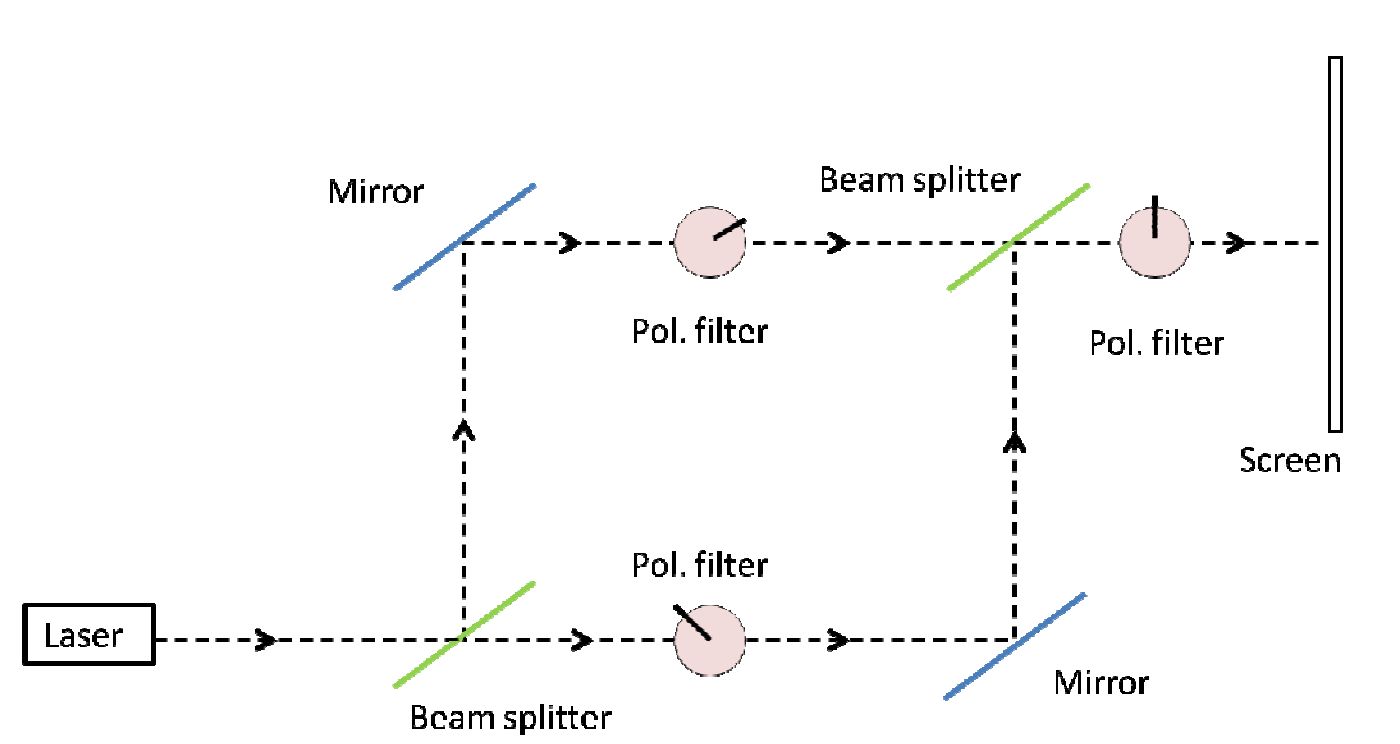
\includegraphics[width=1\textwidth]{pics/schema.png}
			\caption{Aufbau eines Mach-Zehnder-Interferometers mit Polarisationsfiltern. \cite{EMAUGreifswaldMAZ}}
			\label{abb:schema}
		\end{figure}
	
	\subsection{Interferenz für Wellen}
	
	Werden die Lichtstrahlen als elektromagnetische Wellen beschrieben, so ist der optische Phasenunterschied zwischen beiden von Bedeutung zur Bestimmung der Interferenz. Hierbei spielen sowohl die Reflexion an Spiegeln als auch das durchlaufen von verschiedenen Medien eine Rolle. Bei der Reflexion erfährt ein Lichtstrahl eine Phasenverschiebung von $\pi$. Dabei müssen nicht nur die Reflexionen an den Spiegeln, sondern auch die an den Strahlteilern berücksichtigt werden.\\Die Strahlteiler seien so aufgestellt, dass der reflektierte Strahl nicht das Trägermaterial der Teilers durchläuft. Demzufolge nimmt der nicht reflektierte Strahl eine zusätzliche Phase von 
	\begin{equation}
		\frac{2\pi t}{\lambda} \nonumber
	\end{equation}
	auf, wobei $t$ die optische Weglänge des Strahles durch das Trägermedium und $\lambda$ die Wellenlänge des Lichtes sind. Bei Betrachtung von \autoref{abb:schema} ist zu erkennen, das die Strahlen bei der Rekombination entweder eine Phasendifferenz von $0$ (wie eingezeichnet) oder eine von $\pi$ (falls der untere Strahl \textbf{nicht} refletiert wird) haben.\\
	Die Strahlen sind nur in der Lage miteinander zu interferieren, wenn sie die gleiche Polarisation haben. Sind sie in einem $90^\circ$ Winkel zueinander polarisiert, so können sie nicht interferieren. Werden die  getrennten Strahlen durch Polarisationsfilter in einem Winkel der kleiner ist linear polarisiert, so kann der Kontrast zwischen Minima und Maxima des Interferenzbildes variiert werden.
	
	\subsection{Interferenz für Photonen}
	
	Licht kann nicht nur als Welle, sondern auch als einzelne quantenmechanische Teilchen, also Photonen, beschrieben werden. Dabei kann das Problem der Interferenz für dieses Experiment auf die Frage reduziert werden: 
	\begin{quote}
		Wählt das Photon einen bestimmten Weg, wird es also vom Strahlteiler entweder durchgelassen oder reflektiert, und zeigt es so seine Teilcheneigenschaft, oder wird es sozusagen gleichzeitig durchgelassen und reflektiert, so dass es mit sich selbst interferiert und seine Wellennatur zeigt? \par\raggedleft ---\text{A. Schimony, Die Realität der Quantenwelt; 1996, S. 75 \cite{MZquote}}
	\end{quote}
	In diesem Teilchenbild ist es nach der Heisenbergschen Unschärferelation nicht möglich festzulegen, welchen Weg das Photon am ersten Strahlteiler einschlägt, woraus folgt, dass schon ein einzelnes Photon immer eine nicht verschwindende Wahrscheinlichkeit besitzt beide Wege des Interferometers zu gehen und dadurch mit sich selber zu interferieren. Das heißt, dass das Photon quantenmechanisch durch eine Superpostion der Zuständen beschrieben werden kann. Gesetzt jedoch dem Falle das sich Polarisatoren auf den einzelnen Wegstrecken befinden, kann genau festgelegt werden, welchen der beiden Wege das Photon genommen hat. Durch diese Messung des Systems wird der vorher Superpositionszustand verändert und das Photon verliert die Möglichkeit auf beiden Wegen gleichzeitig zu existieren und somit kann es nicht mit sich selber interferieren. Wird nun noch ein Polarisator hinter dem zweiten Strahlteiler in den rekombinierten Strahl gesetzt, so wird diese vorher festgelegte Information {}"ausradiert{}" und es kann wieder ein Interferenzmuster am Schirm beobachtet werden. Dieses Phänomen wird entsprechend als Quantenradierung bezeichnet.
	
	
	\newpage
	\section{Durchführung}
	
	Der Versuch wird in drei Schritten durchgeführt. Dabei wird sich für den Aufbau und die Beschriftungen auf \autoref{img:aufbau2} bezogen. Im ersten Schritt wird die Polarisation des Laser und das $\lambda /4$-Plättchen (\textbf{quater lamda}) geprüft. Dafür wird das Laserlicht zuerst durch einer der Polarisatoren gestrahlt und der Polarisationswinkel variiert. Das die Intensität der transmitierten Lichtes wird über den Stromfluss einer Photodiode gemessen. Diese Messung wird wiederholt für einen zweiten Polarisator, welcher hinter den ersten angebracht wird, wobei jetzt der Winkel des ersten fest ist. Anschließend wird die Messung mit dem $\lambda/4$-Plättchen durchgeführt. Im zweiten Schritt wird das Mach-Zehnder-Interferometer nach \autoref{img:aufbau2} aufgebaut. Hierbei ist zu beachten, das die Höhe des Laserstrahls ab besten an den Spiegeln \textbf{M1} und \textbf{M2} eingestellt wird und die Vertikale Position sowohl an \textbf{einen} der Spiegel \textbf{M3} oder \textbf{M4} als auch am zweiten Strahlteiler \textbf{BS2} eingestellt wird. Bei der Justierung sollten die Linse \textbf{Lens} und das $\lambda/4$-Plättchen eingebaut sein um den Strahl aufzuweiten und an einer weit entfernten Projektionsfläche die Optimierung des Interfenzmusters überprüfen zu können. Zum Schluss können die Polarisatoren eingesetzt werden. Im letzten Schritt werden mit einer CCD-Kamera werden anschließend Interferenzmuster auf den Bildschirm \textbf{SC2} für verschiedene Polarisationswinkel aufgenommen.
	
	\begin{figure}[H]
		\centering
		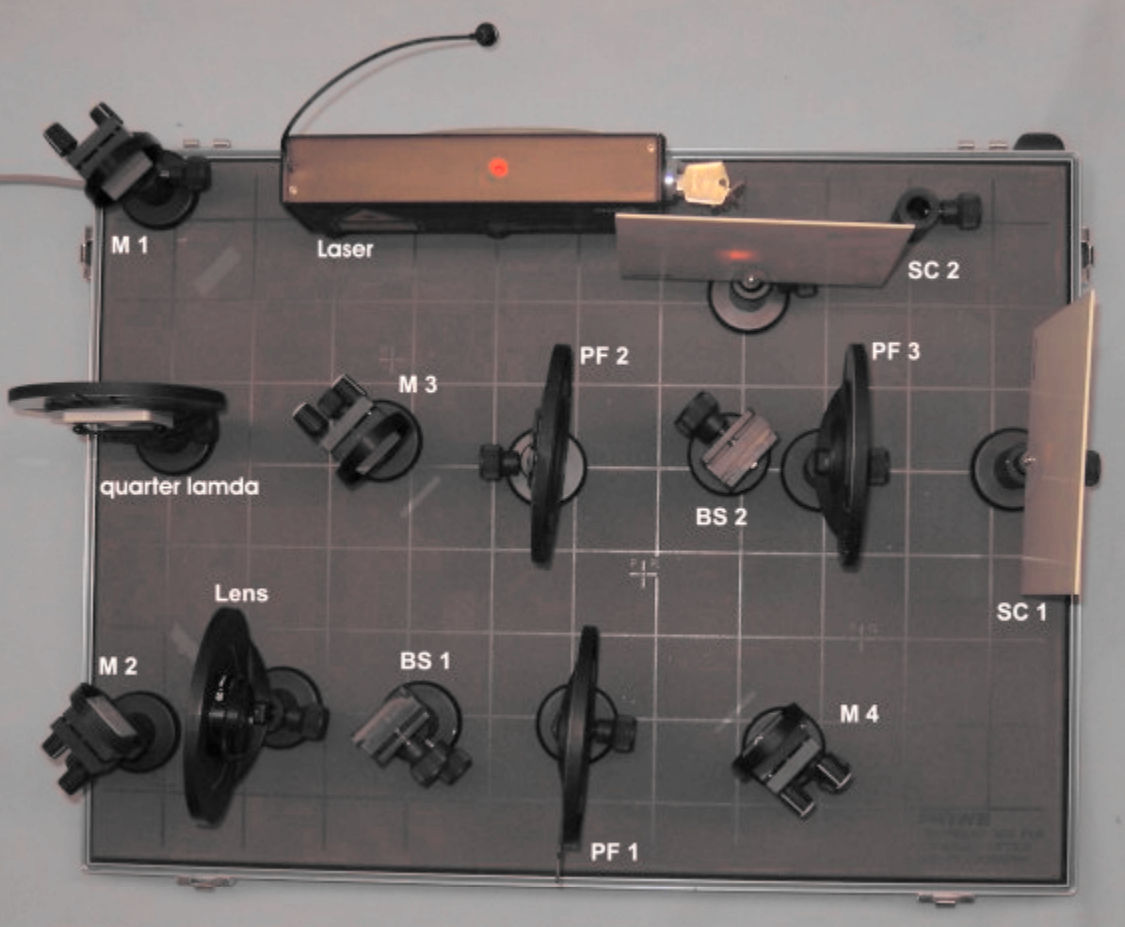
\includegraphics[width=0.85\textwidth]{pics/aufbau.png}
		\caption{Aufbau des finalen Experimentes nach \cite{MZaufbau}. Das $\lambda/4$-Plättchen entspricht dem \tilt{quarter lambda}, die Spiegel den \fett{M1} bis \fett{M4} und die Strahlteiler den \fett{BS1} und \fett{2}. Beobachtet wird die Intereferenz auf \fett{SC1} und \fett{SC2}.}
		\label{img:aufbau2}
	\end{figure}
	
	\newpage
	\section{Auswertung}

\subsection{Polarisationsgrad des Laserlichtes}

Zur Bestimmung der Polarisation wird die Intensität des durch einen Polarisator transmitierten Laserlichtes gemessen. Die aufgenommenen Werte sind in \autoref{fig:1xpol} dargestellt. Die Intensität weist bei kleinen Winkeleinstellungen auf. Weiterhin ist zu beobachten, dass die Intensität in beide Richtungen gleichermaßen abnimmt, bis sie jeweils bei einem Winkel von ca. $90^\circ$ in ein Minimum läuft. Um den Polarisationgrad zu bestimmen kann die Beziehung
\begin{equation}
	K = \frac{I_\mathrm{max}-I_\mathrm{min}}{I_\mathrm{max}+I_\mathrm{min}}
	\label{eq:kontrast}
\end{equation}
verwendet werden, welche den Kontrast $K$ in Abhängigkeit der minimalen und maximalen Intensität $I_\mathrm{max}$, $I_\mathrm{min}$ setzt. Je höher der gemessene Kontrast ist, desto näher ist das Licht total Polarisiert. Für diese Messung wird als minimale Intensität ein Wert von $I_\mathrm{min} = 0,2$ und als maximale Intensität $I_\mathrm{max} = 33,0$ aufgenommen. Der zugehörige Kontrast ist $K \approx 0,99$, weshalb man von quasi vollständig polarisierten Laserlicht ausgehen kann.

\begin{figure}[h]
	\centering
	\begin{subfigure}{.49\textwidth}
		\centering
		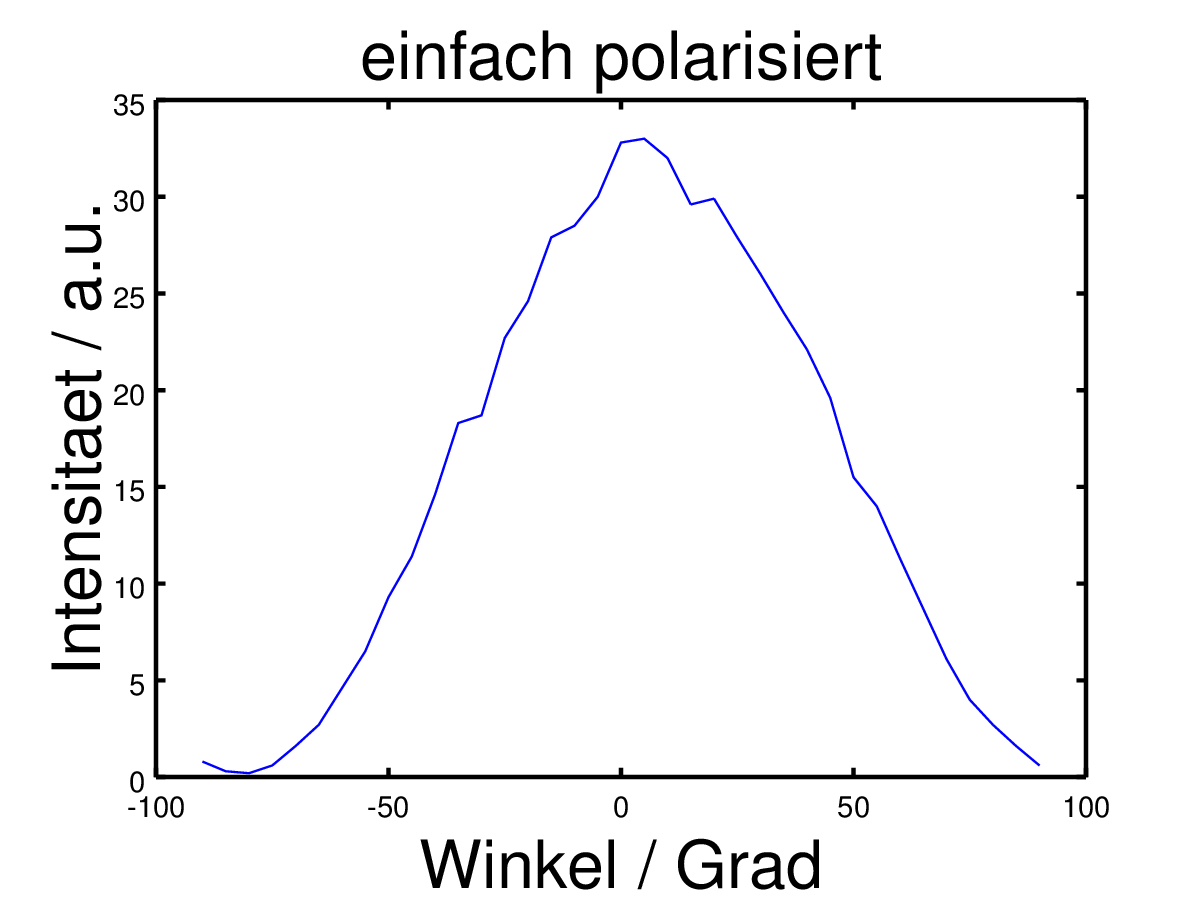
\includegraphics[width=0.8\linewidth]{pics/1xpol.png}
	\end{subfigure}
	\begin{subfigure}{.49\textwidth}
		\centering
		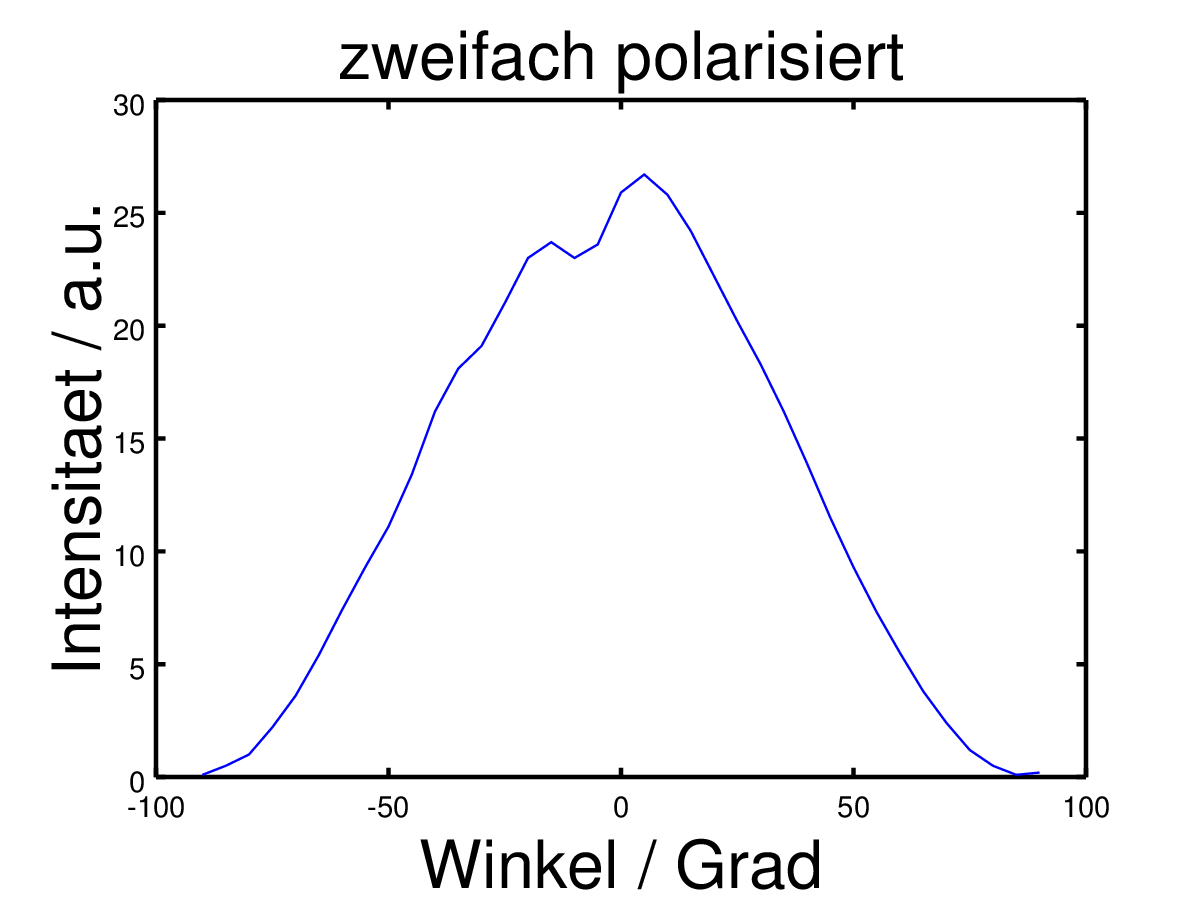
\includegraphics[width=0.8\linewidth]{pics/2xpol.png}
	\end{subfigure}
	\caption{Intensität des Laserlichtes nach dem Durchgang eines bzw. zwei Polarisatoren in Abhängigkeit der Einstellungsinkel.}
	\label{fig:1xpol}
\end{figure}

Weiterhin sind ist der Intensitätsverlauf des Lichtes nach Durchgang durch das $\lambda/4$-Plättchen und eines auf $0^\circ$ eingestellten Polarisators in Abhängigkeit des Einstellungswinkels des Plättchens in \autoref{fig:lambda4} dargestellt. Die Messung zeigt, das dass $\lambda /4$-Plättchen, nicht wie erwartet bei $45^\circ$ zirkular polarisiertes Licht erzeugt, sondern bei einem Winkel von ca. $50^\circ$. Für die weiteren Messung wird diese Einstellung verwendet. \clearpage

\begin{figure}[h]
	\centering
	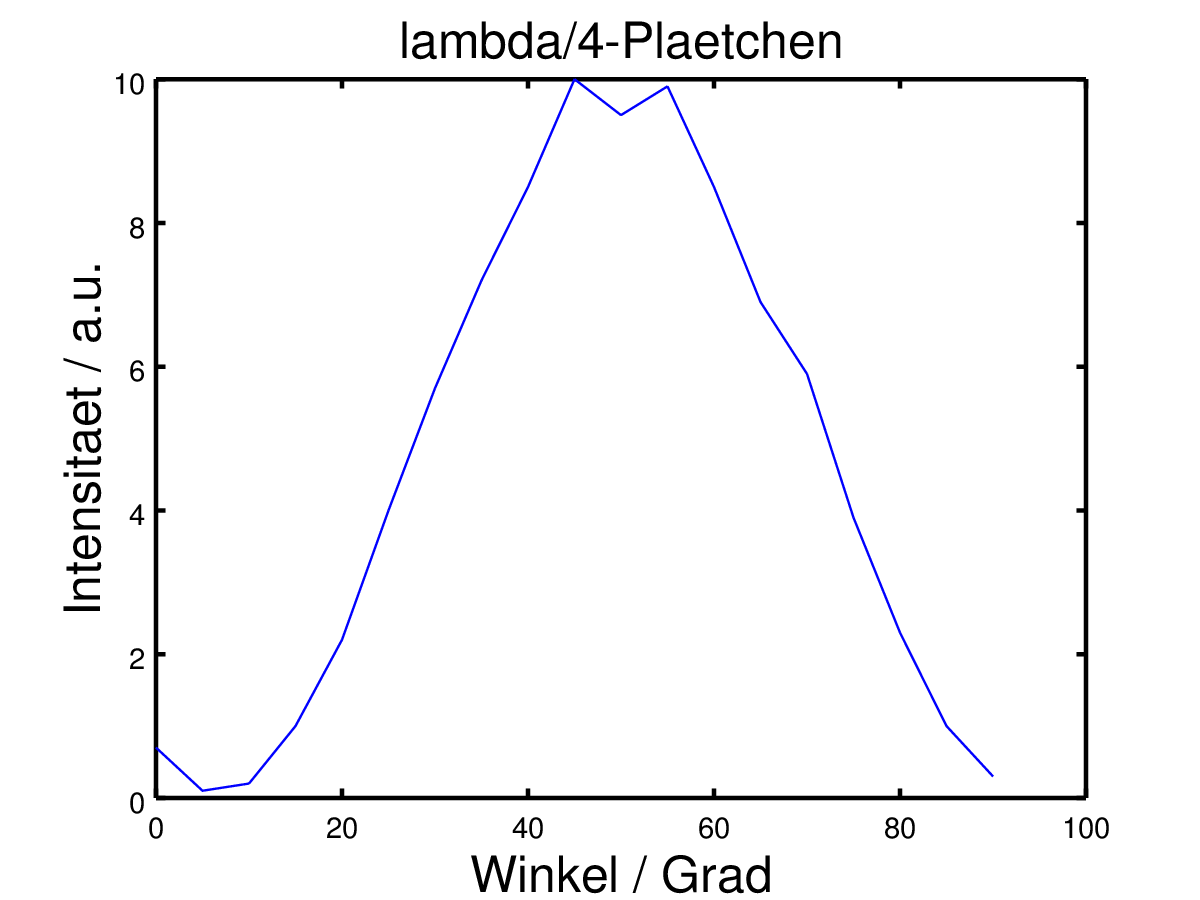
\includegraphics[width=0.5\columnwidth]{pics/lambda4.png}
	\caption{Intensität des Laserlichtes nach dem Durchgang durch das $\lambda /4$-Plättchen und einen auf $0^\circ$ eingestellten Polarisator. Bei der Messung wurde der Einstellungswinkel des $\lambda /4$-Plättchens variiert.}
	\label{fig:lambda4}
\end{figure}

\subsection{Kontrastfunktion des Mach-Zehnder-Interferometers}	

Nach dem Aufbau des Mach-Zehnder-Interferometers wird das Interferenzmuster mit einer Kamera aufgenommen. Dieses ist ohne einsetzen der Polarisatoren in \autoref{fig:ohnealles} dargestellt. Es war im Zeitrahmen des Versuches nicht möglich ein Interfenzmuster mit Ringen zu erzeugen und es wurde sich mit den dargestellten Muster zufrieden gegeben. 

\begin{figure}[h]
	\centering
	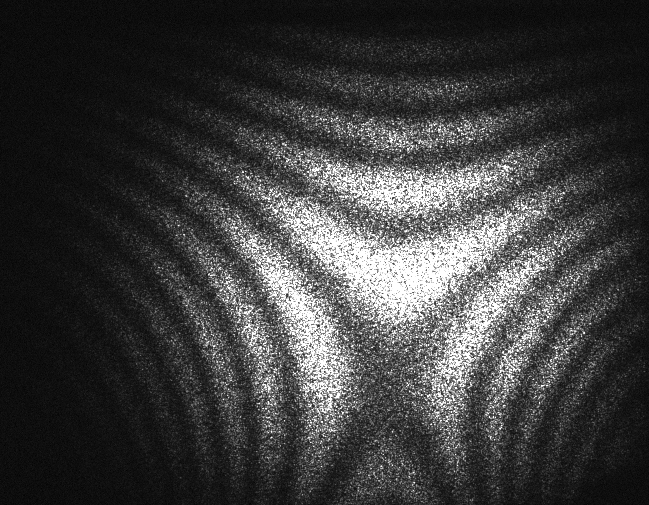
\includegraphics[width = 0.5 \columnwidth]{pics/ohnealles.png}
	\caption{Interferenzmuster des rekombinierten Laserlichtes an einem der Schirme aufgenommen mit einer CCD Kamera in Graustuffen.}
	\label{fig:ohnealles}
\end{figure}

Nach dem Einbau der Polarisatoren werden Aufnahmen bei verschiedenen Einstellungswinkel vorgenommen, wobei der Winkel von $0^\circ$ bis $90^\circ$ in $5^\circ$ Schritten variiert wird. In \autoref{fig:interpol} sind die Interferenzmuster vom minimalen und maximalen Winkel zur Veranschaulichung gegenüber gestellt. Ein Querschnitt durch diese Bilder ist in \autoref{fig:test} für ausgewählte Winkel dargestellt. Der Querschnitt wurde hierbei für jeden Fall an der gleichen Stelle angefertigt. Es ist bereits mit dem Auge zu erkennen, das der Kontrast bei größeren Winkeln abnimmt und für die Messung bei $90^\circ$ ist bereits kein Interferenzmuster mehr zu erkennen. An Hand der Querschnitte kann mit Hilfe von \autoref{eq:kontrast} der Kontrastverlauf der Messung aufgetragen werden. Das Ergebnis ist in \autoref{fig:kontrast} dargestellt.

\begin{figure}
	\centering
	\begin{subfigure}{.49\textwidth}
			\centering
			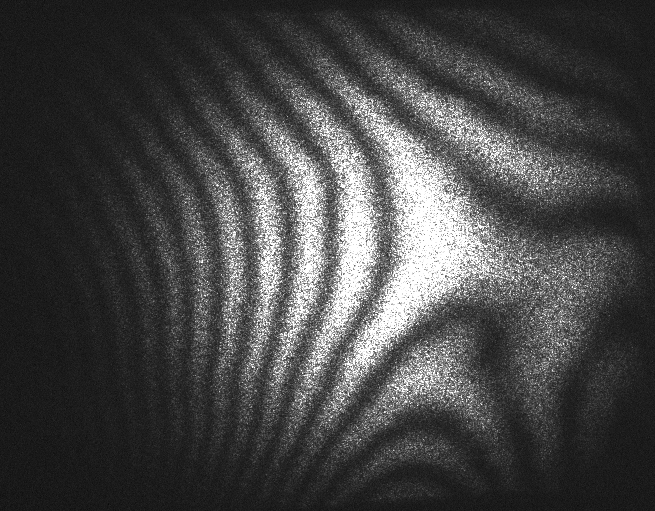
\includegraphics[width=.7\linewidth]{pics/0grad_.png}
	\end{subfigure}
	\begin{subfigure}{.45\textwidth}
		\centering
		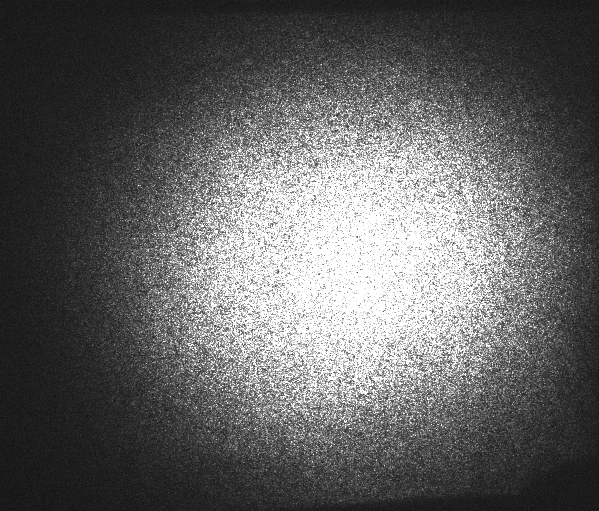
\includegraphics[width=.7\linewidth]{pics/90grad_.png}
	\end{subfigure}	
	\caption{Interfentmuster des rekombinierten Laserlichtes nach dem Einsetzten der Polarisatoren bei einer Winkeleinstellung von $0^\circ$ bzw. $90^\circ$ in Graustuffen.}
	\label{fig:interpol}
\end{figure}


\begin{figure}
	\centering
	\begin{subfigure}{.49\textwidth}
		\centering
		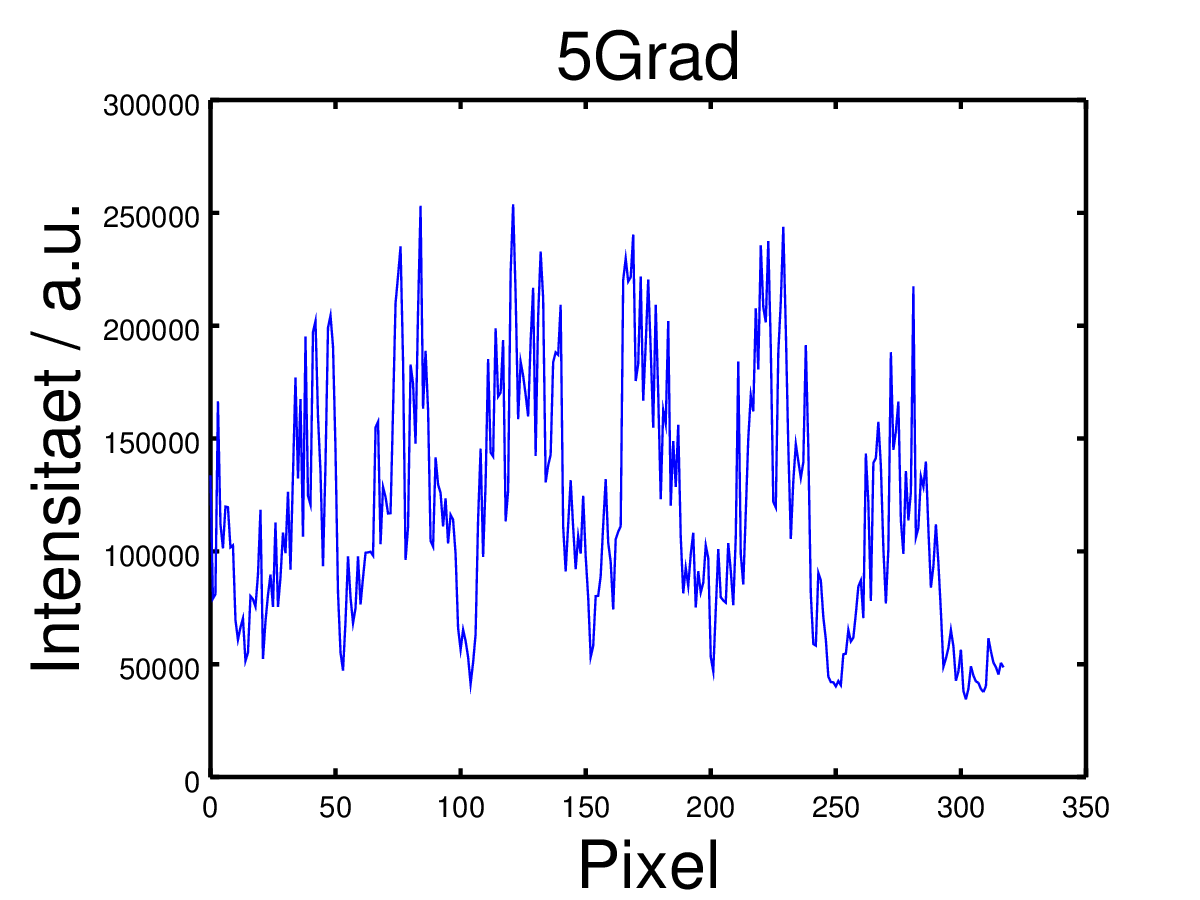
\includegraphics[width=0.75\linewidth]{pics/5grad.png}
	\end{subfigure}
	\begin{subfigure}{.49\textwidth}
		\centering
		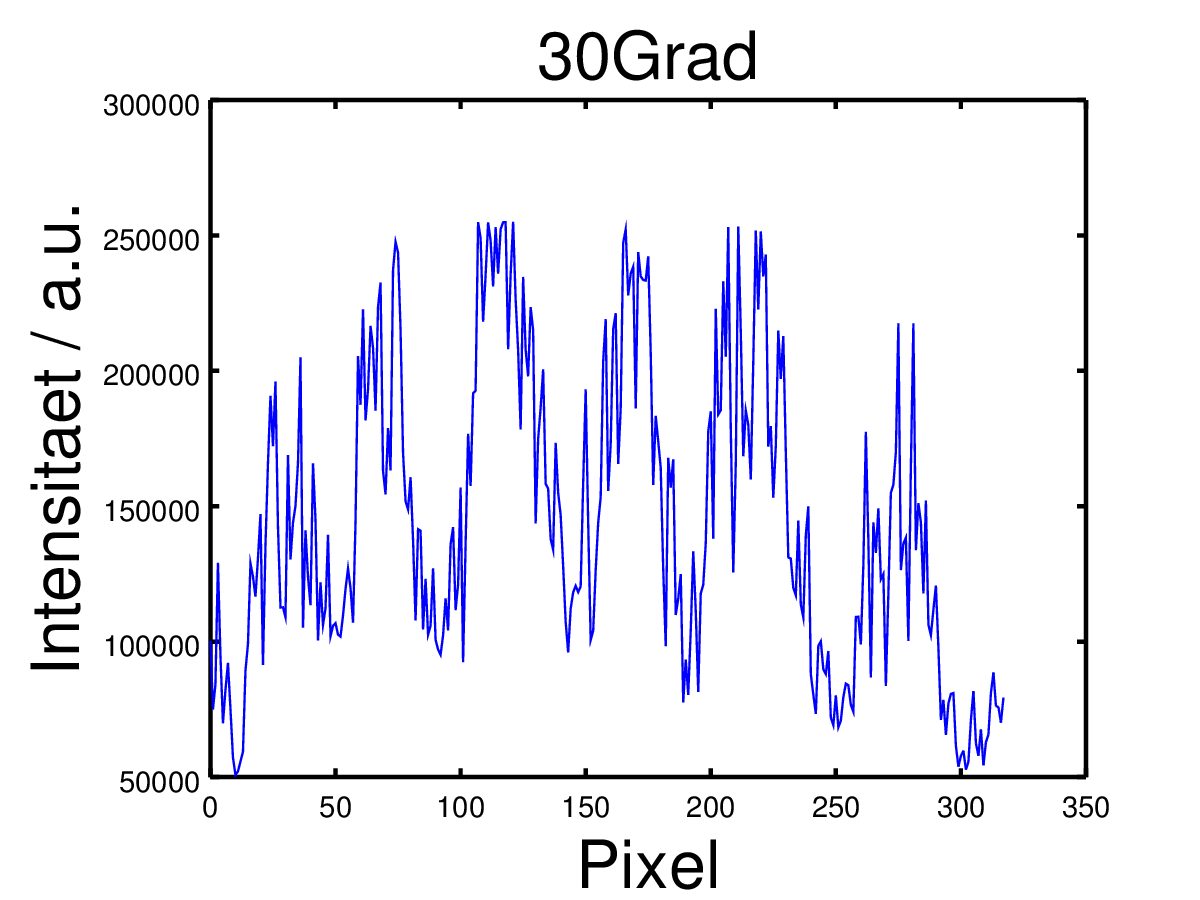
\includegraphics[width=0.75\linewidth]{pics/30grad.png}
	\end{subfigure}
	\begin{subfigure}{.49\textwidth}
		\centering
		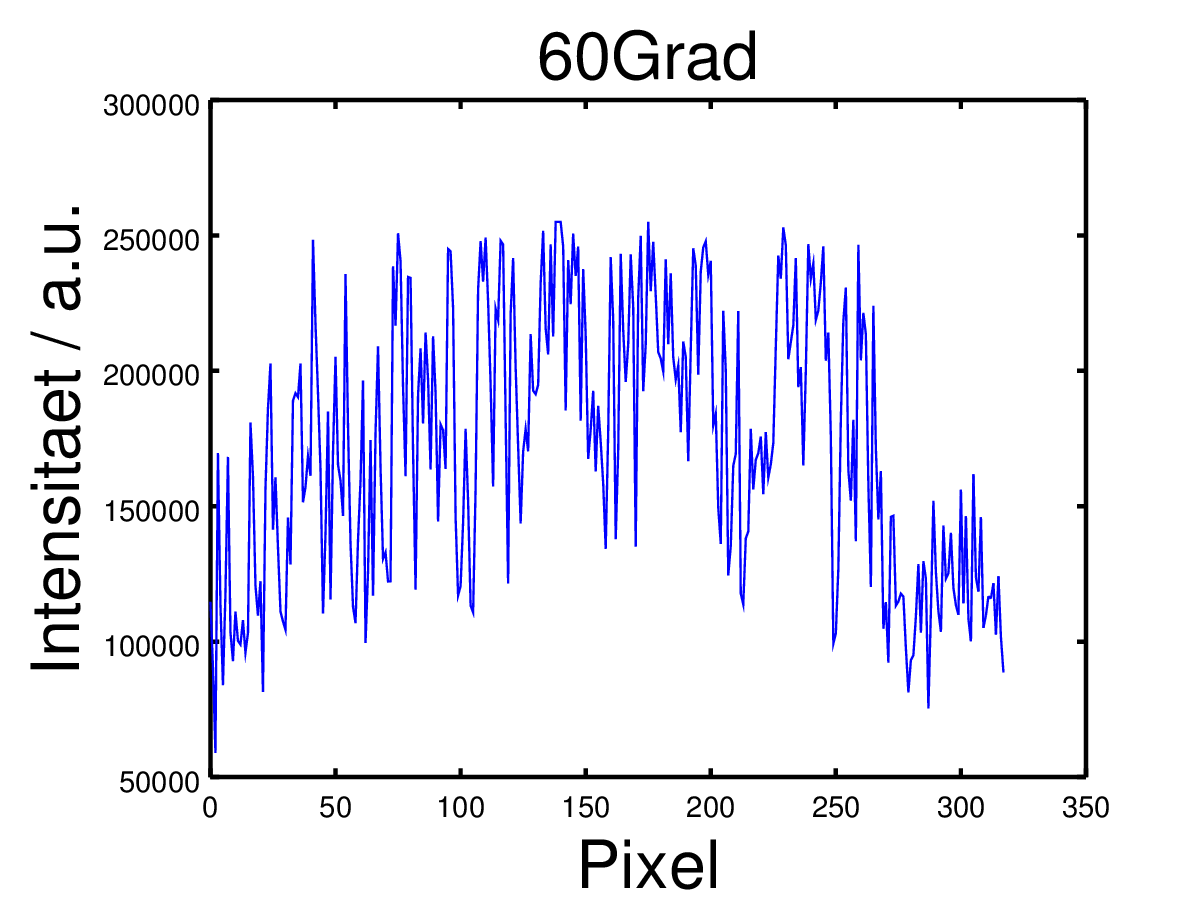
\includegraphics[width=0.75\linewidth]{pics/60grad.png}
	\end{subfigure}
	\begin{subfigure}{.49\textwidth}
		\centering
		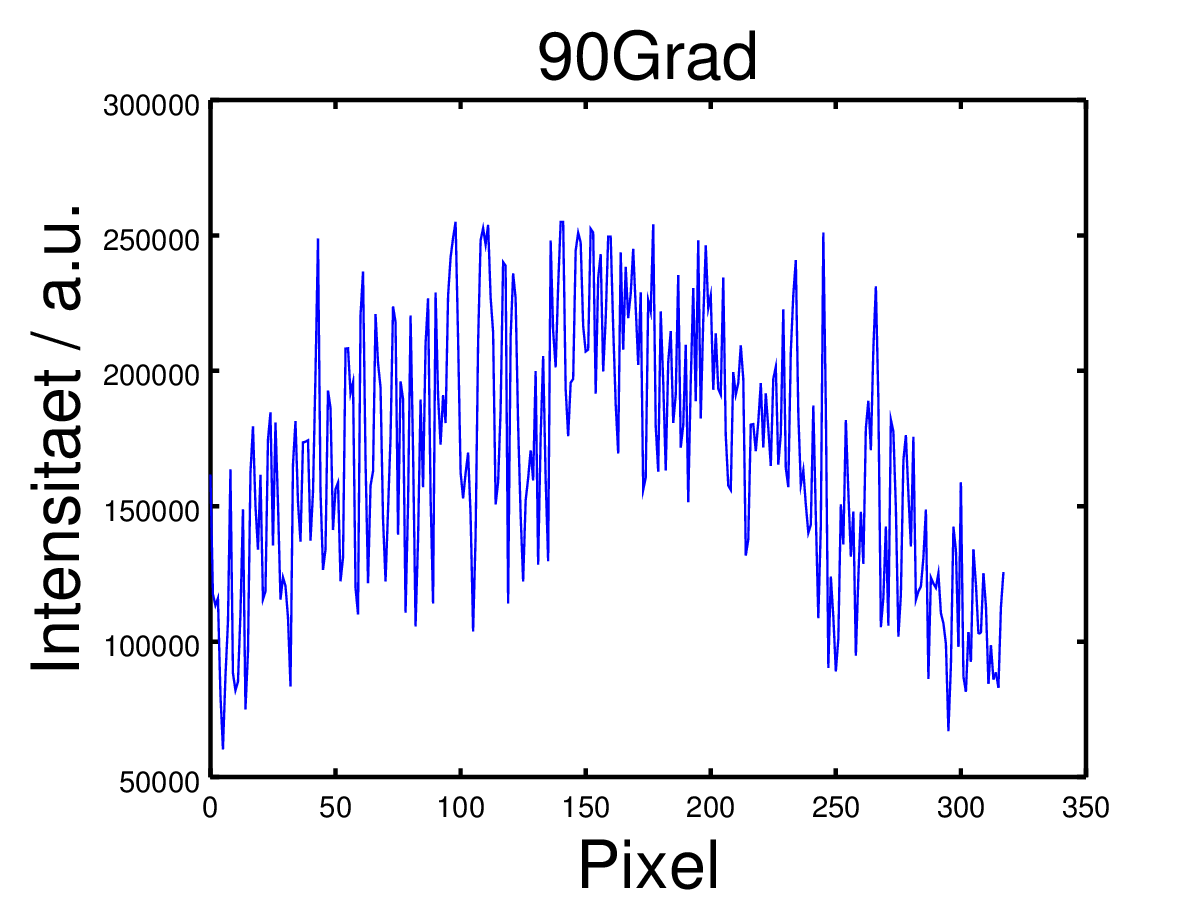
\includegraphics[width=0.75\linewidth]{pics/90grad.png}
	\end{subfigure}
	\caption{Intensitätsprofil des Interferenzmusters entlang einer Graden für verschiedene Winkeleinstellung des Polarisators.}
	\label{fig:test}
\end{figure}

\begin{figure}
	\centering
	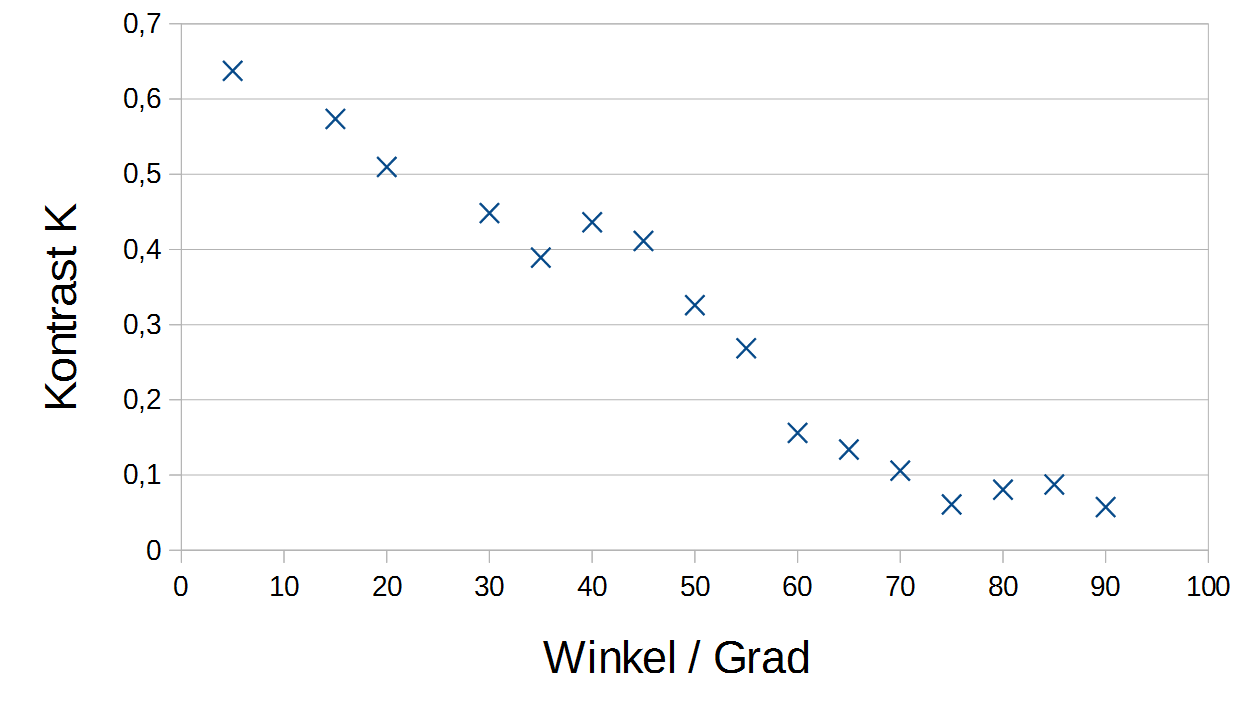
\includegraphics[width=0.8\columnwidth]{pics/Kontrast.png}
	\caption{Kontrast des Interfenzmusters in Abhängigkeit des Einstellungswinkels des Polarisators.}
	\label{fig:kontrast}
\end{figure}
\newpage
\subsection{Diskusion der Ergebnisse}

Der Kontrastverlauf in \autoref{fig:kontrast} fällt zwar mit zunehmenden Winkel ab, schwankt aber stark. Der Hauptgrund für diese Schwankungen ist eine schlechte Belichtung der Aufnahme. Die intensivsten Maxima in den Bildaufnahmen sind stark überbelichtet und übersteigen das Maximum der Intensität, welche einen arbiträren Zahlenwert von $255$ hat. Dadurch kann der Kontrast nicht im Zentrum des Bildes gemessen werden, sondern wird möglichst nahe am diesem angesetzt. Diese Intensitätsprofile haben jedoch starke Schwankungen, wodurch der Kontrast für die einzelnen Winkeleinstellungen nur approximativ bestimmt werden kann.\\
Weiterhin konnte im Zeitrahmen des Versuches der Aufbau des Quantenradierers nicht mehr realisiert werden, wodurch eine Auswertung einer solchen Messung ausbleibt.
	
	\newpage
	\section{Anhang}

		\bibliography{all.bib}
		\bibliographystyle{unsrt}

\end{document}